\documentclass[]{beamer}

%%
%% RWTH Beamer Theme (layout based on RWTH PowerPoint template)
%% by Georg Wassen, Lehrstuhl für Betriebssysteme, 2013
%%    wassen@lfbs.rwth-aachen.de
%% with modifications by Gerrit Toehgiono, Mentoring Informatik, 2016-2018
%% to match the "current old" RWTH template
%%
%% The templates are derived from the beamer documentation and the provided templates,
%% hence, the same licence applies:
%%
%% ----------------------------------------------------------------
%% |  This file may be distributed and/or modified                |
%% |                                                              |
%% |  1. under the LaTeX Project Public License and/or            |
%% |  2. under the GNU Public License.                            |
%% |                                                              |
%% |  See the file doc/licenses/LICENSE for more details.         |
%% ----------------------------------------------------------------
%%
%% Version 0.1    20.12.2012    Initial presentation using this theme
%% Version 0.2    08.01.2013    Extracted layout and some example slides
%% Version 0.3    12.01.2013    Improved handling of \subsection (used as frame title),
%%                              Support institute's logo
%% Version 0.4    22.01.2013    Improved spacing between lines in header & footer
%% Version 0.5    01.02.2013    No right sidebar: set width correctly
%% Version 1.0    06.03.2014    Initial Tag on GitHub
%%
%% Version 1.1    31.03.2018    Modifications for CS Mentoring
%%
%% TODO
%%  - copyright of slides?
%%  - count slides with same subsection (needs probably overloading \subsection) and print: 1/N
%%    (needs to count the number of frames in each subsection)

%%%%%%%%%%%%%%%%%%%%%%%%%%%%%%%%%%%%%
%% Select input file encoding:
%%   utf8   - UTF-8, nowadays standard on most operating sytems
%%   latin1 - ISO-8859-1
\usepackage[utf8]{inputenc}

%%%%%%%%%%%%%%%%%%%%%%%%%%%%%%%%%%%%%
%% Select language
%%
\usepackage[ngerman]{babel}        % Deutsch, neue Rechtschreibung
%\usepackage[english]{babel}       % English

\usetheme{rwth}
\usepackage[T1]{fontenc}           % Font encoding (don't change!)
\usepackage{lmodern}               % Select Linux Modern Fonts (don't change)
\usepackage{sansmathfonts}         % Sans fonts in math environments
\usepackage{textcomp}              % fix 'missing font symbols' warning
\renewcommand{\rmdefault}{phv}     % Arial like (Helvetica)
\renewcommand{\sfdefault}{phv}     % Arial like (Helvetica)

%% graphics related packages
\usepackage{graphicx}              % needed to include graphics (don't change)
\usepackage{epstopdf}              % required to include eps files
%\usepackage{svg}                   % include svg files (requires Inkscape)
\usepackage[encoding,filenameencoding=utf8]{grffile} % allow utf8 file names in graphics

%%%%%%%%%%%%%%%%%%%%%%%%%%%%%%%%%%%%%
%% import packages for content
%%
\usepackage{listings}                           % for lstlisting and \lstinline|..|
%% TikZ can be used to /program/ graphics.
\usepackage{tikz}                                % comment-out, if you don't need this.
%% some TikZ-libraries and settings for the examples...
\usetikzlibrary{shadings}           % GW: color gradients
\usetikzlibrary{arrows,calc,positioning,fit,matrix,shadows,chains,arrows,shapes,spy,fadings}
\usepackage{pgfplots}
\usetikzlibrary{pgfplots.units,shapes.symbols,shapes.arrows}
%\usetikzlibrary{pgfplots.external}
%\tikzexternalize[prefix=tmp/]

%% Custom packages and definitions
\usepackage{minted}
\usepackage{csquotes}
\usepackage{bbding}

% Mathematikumgebung
\usepackage{amsmath}
\usepackage{amssymb}
\usepackage{sansmath}

% tabularx -> bessere "tabular"-Umgebung
\usepackage{tabularx}

% zusätzliche Formatbezeichner für die tabularx-Umgebung
\newcolumntype{L}{>{\raggedright\let\newline\\\arraybackslash\hspace{0pt}}X}
\newcolumntype{R}{>{\raggedleft\let\newline\\\arraybackslash\hspace{0pt}}X}
\newcolumntype{C}{>{\centering\let\newline\\\arraybackslash\hspace{0pt}}X}

% center text vertically in tabularx(column)
%\renewcommand{\tabularxcolumn}[1]{>{\large}m{#1}}

% Bessere Tabellenlinien
\usepackage{booktabs}

% Tabellenzeilen für booktabs anpassen -> call on frame with table
\newcommand{\fixbooktabsrowhight}{%
  \setlength{\aboverulesep}{0pt}
  \setlength{\belowrulesep}{0pt}
  \setlength{\extrarowheight}{.5ex}
}

% Zellen über mehrere Zeilen
\usepackage{multirow}

% Source, e.g. for images
\setbeamercolor{framesource}{fg=gray}
\setbeamerfont{framesource}{size=\tiny}

\usepackage[absolute,overlay]{textpos}
\newcommand{\source}[1]{\begin{textblock*}{\linewidth}(1ex,\paperheight-2.75em)
    \begin{beamercolorbox}[left]{framesource}
      \usebeamerfont{framesource}\usebeamercolor[fg]{framesource} Source: {#1}
    \end{beamercolorbox}
  \end{textblock*}}

\usepackage{etoolbox}
%% short titles for toc \(sub)section[SHORTTITLE for toc]{LONGTITLE for slide}
\makeatletter
% Insert [short title] for \section in ToC
\patchcmd{\beamer@section}{{#2}{\the\c@page}}{{#1}{\the\c@page}}{}{}
% Insert [short title] for \section in Navigation
\patchcmd{\beamer@section}{{\the\c@section}{\secname}}{{\the\c@section}{#1}}{}{}
% Insert [short title] for \subsection in ToC
\patchcmd{\beamer@subsection}{{#2}{\the\c@page}}{{#1}{\the\c@page}}{}{}
% Insert [short title] for \subsection  in Navigation
\patchcmd{\beamer@subsection}{{\the\c@subsection}{#2}}{{\the\c@subsection}{#1}}{}{}
\makeatother



% include config
%%%%%%%%%%%%%%%%%%%%%%%%%%%%%%%%%%%%%
%% configure title page and author information
%%-------------------------------
%% You can always provide a short version: \title[short]{long title}
%%   title        -- Title of the presentation
%%                   The title appears on the first page and may contain a line break: \\ 
%%                   The short title appears in the footer line
%%   subtitle     -- Appears below the title
%%   titlegraphic -- Currently not supported
%%   author       -- Name of the author(s)
%%   email        -- E-Mail address of author (optional)
%%   institute    -- Name of the institution (e.g. chair)
%%   webaddress   -- Web address (default is www.rwth-aachen.de), displayed on last slide
%%   date         -- Date of the presentation (or use \date to insert the date of the PDF generation)
%%   subject      -- This is only for the PDF meta data
%%   keywords     -- This is only for the PDF meta data
%%   logo         -- header Logo, don't change (given by coporate identity templates)
%%   instlogo     -- Logo of institute/chair, if given: will be shown in foot line
\title[RWTH presentation template]{C++20 Ranges und Constrained Algorithms}
% \subtitle{Subtitle}
%\titlegraphic{}
\author{Felix Racz, Tim Wende}
\webaddress{github.com/tmwnd/adv_cpp_seminar} % overrides www.rwth-aachen.de
\date{\today}
\subject{Advanced C++}
% \keywords{RWTH, Latex Beamer, template}

%\logo{
\includegraphics[height=8mm]{logos/logo}} % will replace the default logo

% official institute logo offset correction
%\logo{\vskip-3.5mm\includegraphics[height=12.5mm]{logos/rwth_mentoring_rgb.eps}\hspace{-2mm}} % optionally
\logo{\vskip+2mm
\includegraphics[width=16mm]{logos/logo.pdf}\hspace{+2mm}} % optionally

% alternative logo position (not recommended)
%\instlogo{\includegraphics[height=10mm]{logos/rwth_mentoring_rgb.eps}} % optionally

%%%%%%%%%%%%%%%%%%%%%%%%%%%%%%%%%%%%%
%% configure template behaviour
%%-------------------------------
%%   secstart -- style of section start
%%               selectable parameters:
%%                 sectitle:  only provides section title
%%                 sectoc:    display section table of contents
%%                 <empty>:   display nothing on section start
\secstart{sectitle}



% disable PDF navigation icons
\setbeamertemplate{navigation symbols}{}

\begin{document}
%%
%% the title slide is generated automatically (at begin document)
%%

% include sections
% ueberblick (5 min)
\section{Überblick}
\begin{frame}[fragile]{Implementierung anderer Programmiersprachen}
\frametitle{Ranges in anderen Programmiersprachen}
\begin{itemize}
\item<1->
    Java:
    \begin{minted}{java}
IntStream.range(0, 10)
         .filter(x -> w%2 == 1)
         .map(x -> x*x)
    \end{minted}
\item<2->
    Python:
    \begin{minted}{python}
map(lambda x: x*x,
    filter(lambda x: x%2 == 1,
        range(10)
    )
)
    \end{minted}
\end{itemize}
\end{frame}

% vorwissen (5 min)
\section{Vorwissen}
\begin{frame}{Iteratoren}

\end{frame}
\begin{frame}{Concepts}
    \begin{center}
        Concepts allow us to control the instantiation of templates\\by testing syntactic conditions.

        \vspace{2.5em}

        It is a compile-time predicate which is true if the given type(s)\\meet the requirements.

        \vspace{2.5em}

        \enquote{SFINAE on steroids}
    \end{center}
\end{frame}

\begin{frame}[fragile]{Concepts - Beispiel}
    \begin{minted}{cpp}
template <typename T>
    requires string_convertible<T>
std::string convert(const T& t) { return t.to_string(); }
    \end{minted}
\end{frame}

% einleitung (10 min)
\section{Einleitung}
\begin{frame}{Zu lange Fehlermeldungen}

\end{frame}
\begin{frame}{Unübersichtlicher Code}

\end{frame}
\begin{frame}[fragile]{(Compiler-) Geschwindigkeitsoptimierung}
    \begin{minted}{cpp}
std::vector<int> v{ 3, 1, 4, 1, 5, ... };

std::find(
    v.begin(), // iterator -> v[0]
    v.end(),   // iterator -> nullptr
    5          // ist immer im vector enthalten
);
    \end{minted}
\end{frame}

\begin{frame}[fragile]{(Compiler-) Geschwindigkeitsoptimierung}
    \begin{minted}{cpp}
std::vector<int>::iterator find(
    std::vector<int>::iterator first,
    std::vector<int>::iterator last,
    const int&                 val
) {
    for (; first != last; ++first)
        if (*first == val) break;
    
    return first;
}
    \end{minted}
\end{frame}

\begin{frame}[fragile]{(Compiler-) Geschwindigkeitsoptimierung}
    \begin{minted}{cpp}
std::vector<int> v{ 3, 1, 4, 1, 5, ... };

std::find(
    v.begin(), // iterator -> v[0]
    ranges::unreachable_sentinal, // == it -> false
    5          // ist immer im vector enthalten
);
    \end{minted}
\end{frame}

\begin{frame}{(Compiler-) Geschwindigkeitsoptimierung}
    \begin{center}
        A sentinel is some type that is \texttt{equality\_comparable\_with} its corresponding iterator, which denotes the end of the range.

        \vspace{2.5em}

        Für diese Beispiel benötigen wir den \texttt{unreachable\_sentinal}.
    \end{center}
\end{frame}

\begin{frame}[fragile]{(Compiler-) Geschwindigkeitsoptimierung}
    \begin{minted}{cpp}
std::vector<int>::iterator find(
    std::vector<int>::iterator     first,
    ranges::unreachable_sentinal_t last,
    const int&                     val
) {
    // first == last -> false
    for (; first != last; ++first)
        if (*first == val) break;
    
    return first;
}
    \end{minted}
\end{frame}

\begin{frame}[fragile]{(Compiler-) Geschwindigkeitsoptimierung}
    \begin{minted}{cpp}
std::vector<int>::iterator find(
    std::vector<int>::iterator     first,
    ranges::unreachable_sentinal_t last,
    const int&                     val
) {
    // first == last -> false
    for (; true; ++first)
        if (*first == val) break;
    
    return first;
}
    \end{minted}
\end{frame}

\begin{frame}[fragile]{(Compiler-) Geschwindigkeitsoptimierung}
    Mit dem bekannten Iterator \texttt{.end()} wird jedes Element des Vectors 2 mal \enquote{angefasst}:
    \begin{itemize}
        \item \mintinline{cpp}{first != last}
        \item \mintinline{cpp}{*first == val}
    \end{itemize}

    \vspace{2.5em}

    Durch Sentinals verringern wir diese Zugriffe um die Hälfte, haben jedoch Probleme, wenn \texttt{val} nicht im Vector enthalten ist.
\end{frame}

% anwendung (35 min)
\section{Anwendung}
\subsubsection{Range Concepts}

\begin{frame}[fragile]{Range Concepts <ranges>}
    \begin{itemize}
        \item<1-> \mintinline{c++}{std::ranges::input_range}
            \begin{itemize} \item \mintinline{c++}{std::cin} \end{itemize}
            % \item<2-> std::ranges::forward\_range
            % \only<2->{\begin{itemize} \item std::forward\_list \end{itemize}}
        \item<2-> \mintinline{c++}{std::ranges::bidirectional_range}
            \begin{itemize} \item \mintinline{c++}{std::list} \end{itemize}
        \item<3-> \mintinline{c++}{std::random_access_range}
            \begin{itemize} \item \mintinline{c++}{std::unordered_map} \end{itemize}
            % \item<5-> std::ranges::contiguous\_range
            % \only<5->{\begin{itemize} \item std::vector \end{itemize}}
        \item<4-> \mintinline{c++}{std::ranges::sized_range}
            \begin{itemize} \item \mintinline{c++}{std::vector} \end{itemize}
    \end{itemize}
\end{frame}

% \begin{frame}[fragile]{Bessere Fehlermeldungen}
%     \begin{minted}[fontsize=\tiny, linenos]{console}
% error_messages.cpp:8:5: error: no matching function for call to object of type 'const std::ranges::__sort_fn'
%     std::ranges::sort(list.begin(), list.end());
%     ^~~~~~~~~~~~~~~~~
% /usr/bin/../lib/gcc/x86_64-linux-gnu/11/../../../../include/c++/11/bits/ranges_algo.h:2025:7:
% note: candidate template ignored: constraints not satisfied [with _Iter = std::_List_iterator<int>, _Sent = std::_List_iterator<int>, _Comp = std::ranges::less, _Proj = std::identity]
%       operator()(_Iter __first, _Sent __last,
%       ^
% /usr/bin/../lib/gcc/x86_64-linux-gnu/11/../../../../include/c++/11/bits/ranges_algo.h:2021:14:
% note: because 'std::_List_iterator<int>' does not satisfy 'random_access_iterator'
%     template<random_access_iterator _Iter, sentinel_for<_Iter> _Sent,
%              ^
% [...]
% 1 error generated.

% \end{minted}
% \end{frame}
\subsubsection{Projection}

\begin{frame}{Projection}
    A \emph{projection} is a unary callable which may ne passed to most algorithms.

    \vspace{2.5em}

    Projections modify the view of the data that the algorithms sees.
\end{frame}

\begin{frame}[fragile]{Projection - Beispiel}
    \begin{minted}{cpp}
struct Pokemon {
    int id;
    std::string name;
    ...
}
struct PokedexEintrag {
    int pokemon_id;
    std::string beschreibung;
}

std::vector<Pokemon> pokemon;
std::vector<PokedexEintrag> pokedex;
    \end{minted}
\end{frame}

\begin{frame}{Projection - Beispiel}
    \textbf{Aufgabe:}

    Finde heraus, ob jedes Pokémon einen PokedexEintrag hat.
\end{frame}

\begin{frame}{Projection - Beispiel}
    \begin{center}
        \textbf{Erster Ansatz:}
    \end{center}
    \begin{enumerate}
        \item<1-> Sortiere alle Pokemon (nach \texttt{id})
        \item<2-> Sortiere alle PokedexEinträge (nach \texttt{pokemon\_id})
        \item<3-> Gehe von oben alle Einträge durch.
            Sobald die eine Liste die andere \enquote{überholt}, gib \texttt{false} zurück.
        \item<4-> Wenn wir am Ende der Listen sind, gib \texttt{true} zurück
    \end{enumerate}
\end{frame}

\begin{frame}[fragile]{Projection - Beispiel}
    \begin{minted}{cpp}
std::sort(pokemon.begin(), pokemon.end(),
    [] (const Pokemon& p1, const Pokemon& p2) {
        return p1.id <= p2.id;
    });

std::sort(pokedex.begin(), pokedex.end(),
    [] (const PokedexEintrag& e1,
        const PokedexEintrag& e2) {
        return e1.pokemon_id <= e2.pokemon_id;
    });
    \end{minted}
\end{frame}

\begin{frame}[fragile]{Projection - Beispiel}
    \begin{minted}{cpp}
std::equal(
    pokemon.begin(), pokemon.end(),
    pokedex.begin(), pokedex.end(),
    [] (const Pokemon& p, const PokedexEintrag& e) {
        return p.id == e.pokemon_id;
    });
    \end{minted}
\end{frame}

\begin{frame}{Projection - Beispiel}
    \begin{center}
        \textbf{Zweiter Ansatz:}
    \end{center}

    \begin{itemize}
        \item Erweitere Iteratoren durch Ranges

              \begin{itemize}
                  \item Ersetze \texttt{.begin()} bzw. \texttt{.end()}
              \end{itemize}
    \end{itemize}
\end{frame}

\begin{frame}[fragile]{Projection - Beispiel}
    \begin{minted}{cpp}
std::ranges::sort(pokemon,
    [] (const Pokemon& p1, const Pokemon& p2) {
        return p1.id <= p2.id;
    });

std::ranges::sort(pokedex,
    [] (const PokedexEintrag& e1,
        const PokedexEintrag& e2) {
        return e1.pokemon_id <= e2.pokemon_id;
    });
    \end{minted}
\end{frame}

\begin{frame}[fragile]{Projection - Beispiel}
    \begin{minted}{cpp}
std::ranges::equal(pokemon, pokedex,
    [] (const Pokemon& p, const PokedexEintrag& e) {
        return p.id == e.pokemon_id;
    });
    \end{minted}
\end{frame}

\begin{frame}{Projection - Beispiel}
    \begin{center}
        \textbf{Dritter Ansatz:}
    \end{center}

    \begin{itemize}
        \item Erweitere Ranges durch Projection

              \begin{itemize}
                  \item Reduziere jedes Pokemon auf einen \texttt{int}
                  \item Reduziere analog jeden PokedexEintrag auf einen \texttt{int}
                  \item Überlasse dem Compiler den Umgang mit diesen primitiven Datentypen
              \end{itemize}
    \end{itemize}
\end{frame}

\begin{frame}[fragile]{Projection - Beispiel}
    \begin{minted}{cpp}
std::ranges::sort(pokemon, std::ranges::less{},
    [] (const Pokemon& p) { return p.id; });

std::ranges::sort(pokedex, std::ranges::less{},
    [] (const PokedexEintrag& e) { return e.pokemon_id; });

std::ranges::equal(pokemon, pokedex,
    std::ranges::equal_to{},
    [] (const Pokemon& p) { return p.id; }
    [] (const PokedexEintrag& e) { return e.pokemon_id; }
);
    \end{minted}
\end{frame}

\begin{frame}{Projection - Beispiel}
    \begin{center}
        \textbf{Finaler Ansatz:}
    \end{center}

    \begin{itemize}
        \item Ersetze \enquote{getter}-Lambdas durch die direkten Attribute
    \end{itemize}
\end{frame}

\begin{frame}[fragile]{Projection - Beispiel}
    \begin{minted}{cpp}
std::ranges::sort(pokemon, std::ranges::less{},
    &Pokemon::id);

std::ranges::sort(pokedex, std::ranges::less{},
    &PokedexEintrag::pokemon_id);

std::ranges::equal(pokemon, pokedex,
    std::ranges::equal_to{},
    &Pokemon::id, &PokedexEintrag::pokemon_id);
    \end{minted}
\end{frame}

\begin{frame}{Projection - Beispiel}
    \begin{center}
        \✨ \ \textbf{Finaler Ansatz:} \ \✨
    \end{center}
\end{frame}

\begin{frame}[fragile]{Projection - Beispiel}
    \begin{minted}{cpp}
std::ranges::sort(pokemon, {},
    &Pokemon::id);

std::ranges::sort(pokedex, {},
    &PokedexEintrag::pokemon_id);

std::ranges::equal(pokemon, pokedex, {},
    &Pokemon::id, &PokedexEintrag::pokemon_id);
    \end{minted}
\end{frame}

\begin{frame}[fragile]{Projection - Beispiel}
    Zusammengefasst:

    \begin{minted}{cpp}
// stl
std::sort(pokemon.begin(), pokemon.end(),
    [] (const Pokemon& p1, const Pokemon& p2) {
        return p1.id <= p2.id;
    });

// ranges
std::ranges::sort(pokemon, {}, &Pokemon::id);
    \end{minted}
\end{frame}
\subsubsection{Views}

\begin{frame}{Views}
    \begin{itemize}
        \item<1-> Views leben in \mintinline{c++}{std::ranges::views}
        \item<2-> Es gibt den alias \mintinline{c++}{std::views}
        \item<3-> Was kennzeichnet Views aus?
            \begin{itemize}
                \item<4-> lazy evaluation
                \item<5-> besitzen Inhalt nicht, referenzieren nur
                \item<6-> constant time copy and move
                \item<7-> einfach und effizient kombinierbar
            \end{itemize}
    \end{itemize}
\end{frame}

%Bemerkung: using directives

\begin{frame}{Views - Beispiel}
    \textbf{Aufgabe:}\\
    Berechne für alle Pokémon des Typs Feuer den BMI

    \vspace{2.5em}

    \begin{center}
        $\text{bmi} = \frac{\text{gewicht}}{\text{groesse}^2}$
    \end{center}
\end{frame}

\begin{frame}[fragile]{Klassisch}
    \begin{minted}[fontsize=\footnotesize]{c++}
std::vector<Pokemon> get_pokemon() {...};
auto pokemon = get_pokemon();
std::vector<int> bmis{};

for (const Pokemon& p : vec) {
    if (p.primaer_typ == "Feuer" || p.sekundaer_typ = "Feuer") {
        int bmi = p.gewicht() / (p.groesse() * p.groesse());
        bmis.push_back(bmi);
    }
}
    \end{minted}
\end{frame}

% TODO old stl

\begin{frame}[fragile]{alte STL}
    \begin{minted}{c++}
std::vector<Pokemon> get_pokemon() {...};
auto pokemon = get_pokemon();
std::vector<double> bmis;

std::copy_if(
    pokemon.begin(), pokemon.end(),
    std::back_inserter(feuer_pokemon),
    hat_typ_feuer_lambda);
std::transform(
    feuer_pokemon.begin(), feuer_pokemon.end(),
    std::back_inserter(bmi),
    bmi_lambda);
    \end{minted}
\end{frame}

\begin{frame}[fragile]{Mit Ranges}
    \begin{minted}[fontsize=\footnotesize]{c++}
std::vector<Pokemon> get_pokemon() {...};
auto pokemon = get_pokemon();
auto hat_typ_feuer = [](const Pokemon &p) {
    return p.primaer_typ == "Feuer" || p.sekundaer_typ = "Feuer";
};
auto bmi = [](const Pokemon &p) {
    return (p.gewicht / (p.groesse * p.groesse()));
};

auto view = transform(filter(vec, hat_typ_feuer), bmi);

\end{minted}
\end{frame}

\begin{frame}[fragile]{Mit Ranges und Pipes}
    \begin{minted}[fontsize=\footnotesize]{c++}
std::vector<Pokemon> get_pokemon() {...};
auto pokemon = get_pokemon();
auto hat_typ_feuer = [](const Pokemon &p) {
    return p.primaer_typ == "Feuer" || p.sekundaer_typ = "Feuer";
};
auto bmi = [](const Pokemon &p) {
    return (p.gewicht / (p.groesse * p.groesse()));
};

auto view = vec | filter(hat_typ_feuer) | transform(bmi);

    \end{minted}
\end{frame}

\begin{frame}[fragile]{Mit Ranges und Pipes}
    \begin{minted}[fontsize=\footnotesize]{c++}
std::vector<Pokemon> get_pokemon() {...};
auto pokemon = get_pokemon();
auto view = vec
| filter([](const Pokemon &p) {
    return p.primaer_typ == "Feuer" || p.sekundaer_typ = "Feuer";
})
| transform([](const Pokemon &p) {
    return (p.gewicht / (p.groesse * p.groesse()));
});

    \end{minted}
\end{frame}

\begin{frame}[fragile]{Dangling Iterator}
    \begin{overlayarea}{\linewidth}{6cm}
        \begin{minted}[]{c++}
std::vector<Pokemon> get_pokemon() {...};

auto pokemon = get_pokemon();
auto it = min_element(
    pokemon, {},
    &Pokemon:groesse
);

std::cout << *it << std::enl;
        \end{minted}
    \end{overlayarea}
\end{frame}

\begin{frame}[fragile]{Dangling Iterator}
    \begin{overlayarea}{\linewidth}{6cm}
        \begin{minted}[]{c++}
std::vector<Pokemon> get_pokemon() {...};

auto it = min_element(
    get_pokemon(), {},
    &Pokemon:groesse
);
std::cout << *it << std::enl;
    \end{minted}
        \begin{onlyenv}<2->
            \begin{minted}{c++}
//error: no match for ‘operator*’
//(operand type is ‘std::ranges::dangling’)
            \end{minted}
        \end{onlyenv}
    \end{overlayarea}
\end{frame}

% \begin{frame}[fragile]{Probleme}
%     \begin{minted}[]{c++}
% using std::ranges;
% std::vector<Pokemon> get_pokemons();

% auto it = find(get_pokemons(), 10, &Pokemon:groesse);
% do_something(*it);
% //error: no match for ‘operator*’
% //(operand type is ‘std::ranges::dangling’)
%     \end{minted}
% \end{frame}

\begin{frame}[fragile]{Dangling View}
    \begin{overlayarea}{\linewidth}{6cm}
        \begin{minted}{c++}
std::vector<Pokemon> get_pokemon() {...};
auto hat_typ_feuer = [](const Pokemon &p) { 
    return p.primaer_typ == "Feuer" || p.sekundaer_typ = "Feuer";
};

auto pokemon = get_pokemon();
auto view = views::filter(pokemon, hat_typ_feuer);
for(const Pokemon& p : view) {
    std::cout << p << std::endl;
}
    \end{minted}
        \begin{onlyenv}<-0>
            \begin{minted}{c++}
//note: candidate: ‘template<class _Range, class _Pred>
//requires (viewable_range<_Range>)
            \end{minted}
        \end{onlyenv}
    \end{overlayarea}
\end{frame}

\begin{frame}[fragile]{Dangling View}
    \begin{overlayarea}{\linewidth}{6cm}
        \begin{minted}{c++}
std::vector<Pokemon> get_pokemon() {...};
auto hat_typ_feuer = [](const Pokemon &p) { 
    return p.primaer_typ == "Feuer"
        || p.sekundaer_typ = "Feuer";
};

auto view = views::filter(get_pokemon(), hat_typ_feuer);
for(const Pokemon& p : view)
    std::cout << p << std::endl;
    \end{minted}
        \begin{onlyenv}<2->
            \begin{minted}{c++}
//note: candidate: ‘template<class _Range, class _Pred>
//requires (viewable_range<_Range>)
            \end{minted}
        \end{onlyenv}
    \end{overlayarea}
\end{frame}


\begin{frame}[fragile]{Dangling View}
    \begin{overlayarea}{\linewidth}{6cm}
        \begin{minted}{c++}
std::vector<Pokemon> get_pokemon() {...};
auto hat_typ_feuer = [](const Pokemon &p) {
    return p.primaer_typ == "Feuer"
        || p.sekundaer_typ = "Feuer";
};
auto get_feuer_pokemon(const std::vector<Pokemon>& p) {
    return p | views::filter(hat_typ_feuer);
}
    
auto view = get_feuer_pokemon(get_pokemon())
for(const Pokemon& p : view)
    std::cout << p << std::endl;
        \end{minted}
        \begin{onlyenv}<2->
            \begin{minted}{c++}
//segfault
            \end{minted}
        \end{onlyenv}
    \end{overlayarea}
\end{frame}

%wann dangling view sinnvoll?

\begin{frame}[fragile]{Dangling View}
    \begin{minted}{c++}
std::string s{" Das Ist Ein Langer String. "};
auto s_view(const std::string& s) {
    [...]
    return std::string_view{s};
}
std::string_view = s_view(s);
auto view = sv
            | filter([](char c) { return c!= ' '; });
for (char c : view) {
    std::cout << c;
} //"DasIstEinLangerString"
    \end{minted}
\end{frame}

\begin{frame}[fragile]{Dangling View}
    \begin{minted}{c++}
std::string s{" Das Ist Ein Langer String. "};
auto s_view(const std::string& s) {
    [...]
    return std::string_view{s};
}
auto view = s_view(s)
            | filter([](char c) { return c!= ' '; });
for (char c : view) {
    std::cout << c;
} //"DasIstEinLangerString"
    \end{minted}
\end{frame}

\begin{frame}{\mintinline{c++}{std::ranges::viewable_range}}
    \begin{center}
        \textbf{Was kann man einem Range adaptor alles übergeben?}
    \end{center}
\end{frame}

\begin{frame}{\mintinline{c++}{std::ranges::viewable_range}}

    \textbf{Alles was eine \mintinline{c++}{std::ranges::viewable_range} ist!}

    \begin{itemize}
        \item<2-> lvalue reference (alles mit einem Namen)
        \item<3-> \mintinline{c++}{std::borrowed_range}
            \begin{itemize}
                \item<4-> Alle views
                \item<5-> Typen mit \mintinline{c++}{std::enable_borrowed_range<T>} true
                    \begin{itemize}
                        \item<6-> \mintinline{c++}{std::span, std::string_view}
                    \end{itemize}
            \end{itemize}
    \end{itemize}
\end{frame}
\begin{frame}{Pipes}

\end{frame}

% aufgaben
\section{Aufgaben}
\begin{frame}{Aufgabe}

\end{frame}

\begin{frame}[fragile]{pokemon.hpp}
    \begin{minted}{cpp}
struct Pokemon; // id, name
struct Entwicklung; // pokemon_id

std::vector<Pokemon> get_pokemon();
std::map<int, Entwicklung> get_entwicklung();
    \end{minted}
\end{frame}

% \begin{frame}[fragile]{Pokemon}
%     \begin{minted}{cpp}
% struct Pokemon {
%     int id;
%     std::string name;
%     double groesse;
%     double gewicht;
%     int generation;
%     Typ primaer_typ;
%     Typ sekundaer_typ;
% };
%     \end{minted}
% \end{frame}

% \begin{frame}[fragile]{Entwicklung}
%     \begin{minted}{cpp}
% struct Entwicklung {
%     int pokemon_id;
%     int level;
%     int item_id;
%     int getragenes_item_id;
%     Tageszeit tageszeit;
% };
%     \end{minted}
% \end{frame}

\begin{frame}[fragile]{pokemon\_q.cpp}
    \begin{minted}{cpp}
auto pokemon = get_pokemon();
auto entwicklungen = get_entwicklung();
    \end{minted}
\end{frame}

\begin{frame}{Tipps}
    Schauen wir uns die gegebenen Daten an:

    \begin{center}
        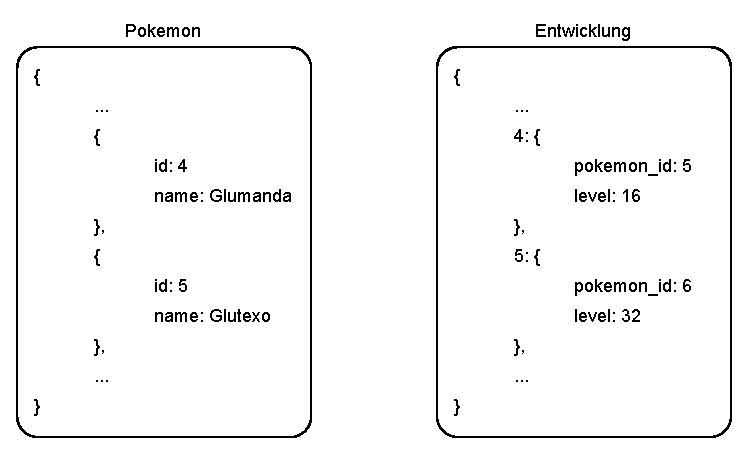
\includegraphics[width=0.75\textwidth]{pictures/example_1.pdf}
    \end{center}
\end{frame}

\begin{frame}{Tipps}
    Zuerst vergleichen wir die n-te \texttt{Pokemon.id} mit \texttt{Entwicklung.von}:

    \begin{center}
        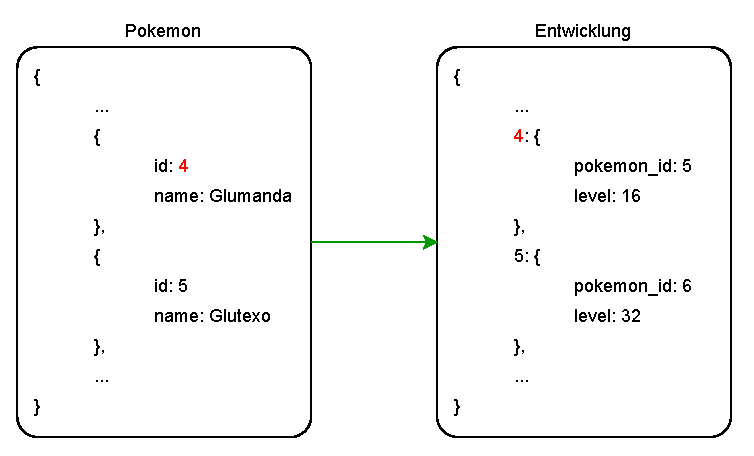
\includegraphics[width=0.75\textwidth]{pictures/example_2.pdf}
    \end{center}
\end{frame}

\begin{frame}{Tipps}
    Die erhaltene \texttt{Entwicklung.zu} finden wir in \texttt{Pokemon.id}:

    \begin{center}
        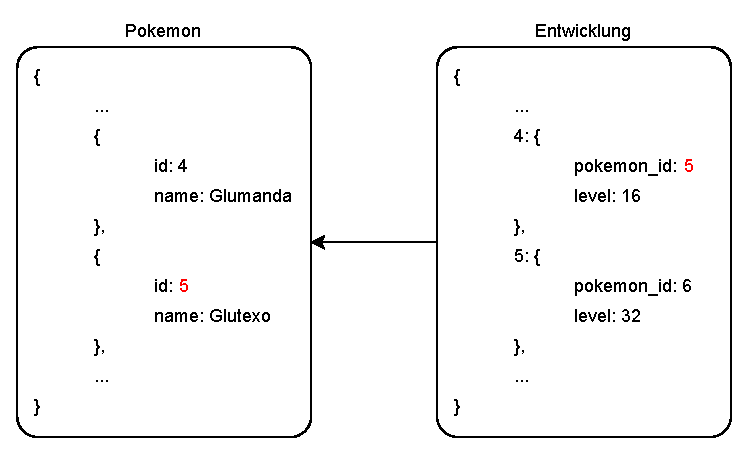
\includegraphics[width=0.75\textwidth]{pictures/example_3.pdf}
    \end{center}
\end{frame}

\begin{frame}{Tipps}
    Nun überschreiben wir das n-te Pokemon mit seiner Entwicklung:

    \begin{center}
        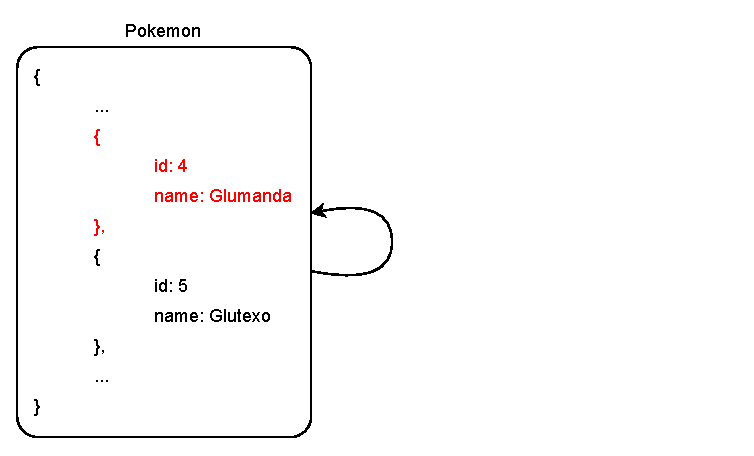
\includegraphics[width=0.75\textwidth]{pictures/example_4.pdf}
    \end{center}
\end{frame}

\begin{frame}{Tipps}
    Und erhalten:

    \begin{center}
        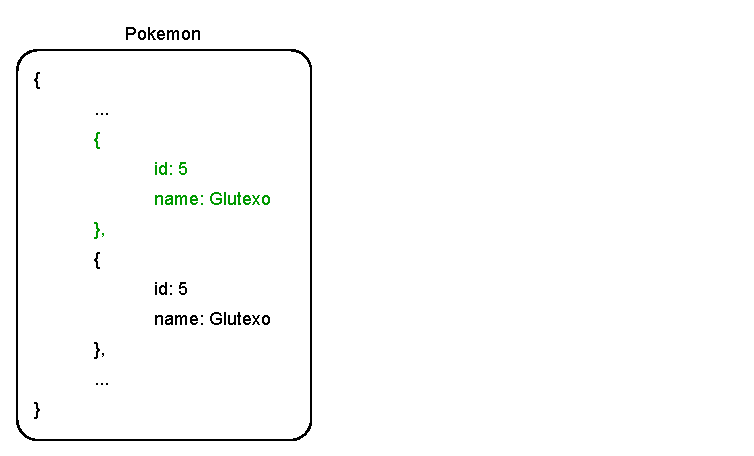
\includegraphics[width=0.75\textwidth]{pictures/example_5.pdf}
    \end{center}
\end{frame}

\begin{frame}{Tipps}
    Sollten wir das n-te Pokemon nicht finden:

    \begin{center}
        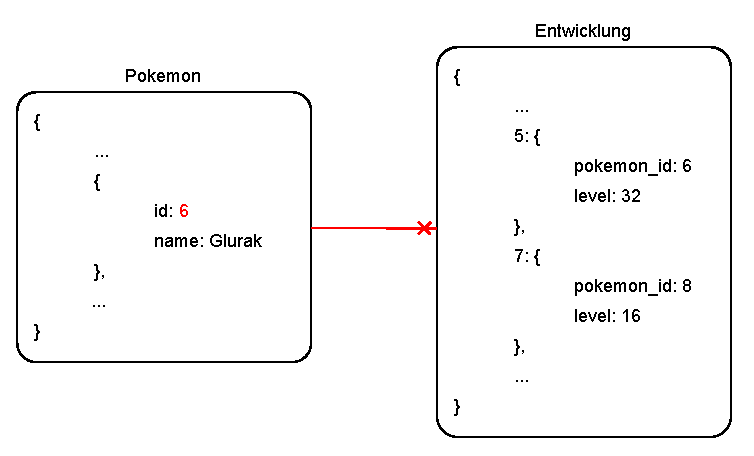
\includegraphics[width=0.75\textwidth]{pictures/example_6.pdf}
    \end{center}
\end{frame}

\begin{frame}{Tipps}
    entfernen wir dieses aus unserer View:

    \begin{center}
        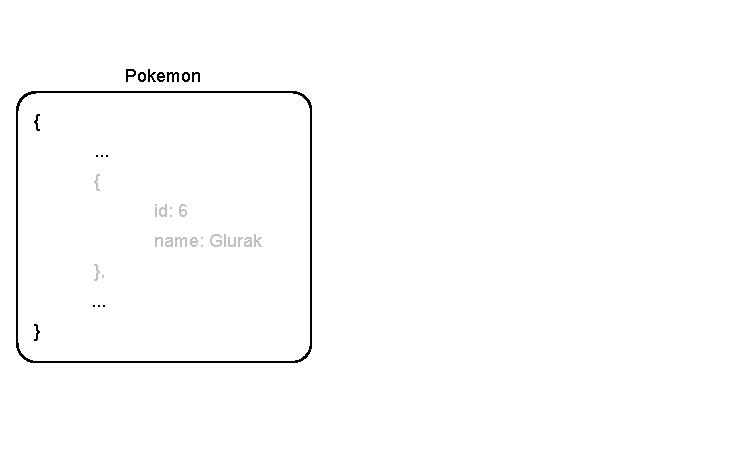
\includegraphics[width=0.75\textwidth]{pictures/example_7.pdf}
    \end{center}
\end{frame}

%quellen
\section*{Quellen}
\begin{frame}{Quellen}
    https://en.cppreference.com/w/cpp/algorithm/ranges
    https://de.wikipedia.org/wiki/Iterator

    \vspace{2em}

    cppcon:\\
    https://www.youtube.com/watch?v=SYLgG7Q5Zws
    https://www.youtube.com/watch?v=d\_E-VLyUnzc
    https://www.youtube.com/watch?v=vJ290qlAbbw
\end{frame}

\end{document}
